% Exercise Template
%A LaTeX template for typesetting exercise in Persian (with cover page).
%By: Zeinab Seifoori

\documentclass[12pt]{exam}

\usepackage{setspace}
\usepackage{listings}
\usepackage{xcolor}

% Define colors
\definecolor{codegreen}{rgb}{0,0.6,0}
\definecolor{codegray}{rgb}{0.5,0.5,0.5}
\definecolor{codepurple}{rgb}{0.58,0,0.82}
\definecolor{backcolour}{rgb}{0.95,0.95,0.92}


% Configure listings style
\lstdefinestyle{mystyle}{
	backgroundcolor=\color{backcolour},   
	commentstyle=\color{codegreen},
	keywordstyle=\color{magenta},
	numberstyle=\tiny\color{codegray},
	stringstyle=\color{codepurple},
	basicstyle=\ttfamily\footnotesize\setLTR,
	breakatwhitespace=true,         
	breaklines=true,                 
	captionpos=top, % Changed to top placement
	keepspaces=true,                 
	numbers=left,                    
	numbersep=5pt,                  
	showspaces=false,                
	showstringspaces=false,
	showtabs=false,                  
	tabsize=2,
	frame=single,
	abovecaptionskip=5pt, % Space between caption and code
	belowcaptionskip=5pt, % Space between code and potential bottom text
}


\lstset{style=mystyle}

% Set Persian caption for listings
\renewcommand{\lstlistingname}{برنامه}

\usepackage{graphicx,subfigure,wrapfig}
\usepackage{float} %for floating shapes

\usepackage{multirow}
%\usepackage{multicol}


%%%%%%%%%  for pie chart %%%%%
\usepackage{pgf-pie}  
%%%%%%%%%%%%%%%%%%%%%%%%%%%%

%%%%%%%% for qoute block %%%%%
\usepackage{etoolbox}
%%%%%%%%%%%%%%%%%%%%%%5


\usepackage[margin=20mm]{geometry}
\usepackage{hyperref}
\hypersetup{
	colorlinks=true,
	linkcolor=blue,
	filecolor=magenta,      
	urlcolor=cyan,
	pdftitle={Overleaf Example},
	pdfpagemode=FullScreen,
}
\usepackage{xepersian}
\settextfont{XB Niloofar}

\newcommand{\class}{درس مبانی هوش محاسباتی}
\newcommand{\term}{نیم‌سال دوم ۰۱-۰۲}
\newcommand{\college}{دانشکده مهندسی کامپیوتر}
\newcommand{\prof}{استاد: دکتر کارشناس}

\onehalfspacing
\parindent 0ex
\begin{document}
	
	
% -------------------------------------------------------
%  Thesis Information
% -------------------------------------------------------

\newcommand{\ThesisType}
{سمینار}  % پایان‌نامه / رساله
\newcommand{\ThesisDegree}
{کارشناسی}  % کارشناسی / کارشناسی ارشد / دکتری
\newcommand{\ThesisMajor}
{مهندسی کامپیوتر}  % مهندسی کامپیوتر
\newcommand{\ThesisTitle}
{تمرین سوم هوش محاسباتی: شبکه های عصبی و کاربردها}
\newcommand{\ThesisAuthor}
{دانیال شفیعی
	
مهدی مهدیه

امیررضا نجفی}
\newcommand{\ThesisSupervisor}
{دکتر کارشناس}
\newcommand{\ThesisDate}
{خرداد ۱۴۰4}
\newcommand{\ThesisDepartment}
{دانشکده مهندسی کامپیوتر}
\newcommand{\ThesisUniversity}
{دانشگاه اصفهان}

% -------------------------------------------------------
%  English Information
% -------------------------------------------------------

\newcommand{\EnglishThesisTitle}{Neural Networks \& Applications}


	\pagestyle{empty}
	
\begin{center}


\includegraphics[scale=0.2]{logo.pdf}

\vspace{0.5cm}
\ThesisUniversity \\[-0.3em]
\vspace{0.5cm}
\ThesisDepartment\\

\begin{large}
\vspace{0.5cm}


%\ThesisMajor

\end{large}

\vspace{1.5cm}

{عنوان:}\\[1.2em]
{\LARGE\textbf{\ThesisTitle}}\\ 
\vspace{1cm}
\begin{latin}
{\Large\textbf\EnglishThesisTitle}
\end{latin}

\vspace{2cm}

{نگارش}\\[.5em]
{\large\textbf{\ThesisAuthor}}

\vspace{1.5cm}

{استاد راهنما}\\[.5em]
{\large\textbf{\ThesisSupervisor}}

\vspace{1cm}



\vspace{2cm}

\ThesisDate

\end{center}

\newpage

	
	% These commands set up the running header on the top of the exam pages
	\pagestyle{head}
	\firstpageheader{}{}{}
	\runningheader{صفحه \thepage\ از \numpages}{}{\class}
	\runningheadrule
	%\begin{tabular}{p{.7\textwidth} l}
	%\multicolumn{2}{c}{\textbf{به نام خدا}}\\
	%\multirow{2}{*}{
\includegraphics[scale=0.2] {images/logo.png}} & \\ \\
	%&  \textbf{\class}\\
	%&  \textbf{\term}\\
	%&  \textbf{\prof}\\ \\
	% \textbf{\college} &  \\
	%\end{tabular}\\
	
	%\rule[1ex]{\textwidth}{.1pt}
	%\textbf{تمرین سری پنجم}
	
	%\rule[1ex]{\textwidth}{.1pt}
	%\makebox[45mm]{\hrulefill}\\
	\tableofcontents
	\vspace{1cm}
	\setcounter{section}{-1}
	\newpage
	\section{مقدمه}
	در این گزارش، پیاده‌سازی یک سیستم کنترل فازی برای آبیاری هوشمند خاک بررسی می‌شود. هدف، نگه‌داشتن رطوبت خاک در محدوده بهینه با توجه به شرایط جوی متغیر است.
	
	\section{پیاده‌سازی}
	
	\subsection{تعریف توابع عضویت}
	برای ورودی‌های \lr{Soil Moisture} (رطوبت خاک)، \lr{Weather Condition} (شرایط جوی) و خروجی \lr{Irrigation Amount} (مقدار آبیاری)، از توابع عضویت مثلثی، ذوزنقه ای و گاوسی کتابخانه \lr{scikit-fuzzy} استفاده شد:
	\newline
	\begin{itemize}
		\item رطوبت خاک:
		\begin{itemize}
			\item خشک: \lr{trapmf([0,0,20,40])}
			\item متوسط: \lr{trimf([30,50,70])}
			\item مرطوب: \lr{trapmf([60,80,100,100])}
		\end{itemize}
		\item شرایط جوی:
		\begin{itemize}
			\item آفتابی: \lr{trapmf([0,0,10,25])}
			\item ابری: \lr{trimf([20,50,80])}
			\item بارانی: \lr{trapmf([60,85,100,100])}
		\end{itemize}
		\item مقدار آبیاری:
		\begin{itemize}
			\item بدون آب: \lr{trapmf([0,0,1,2])}
			\item کم: \lr{trimf([1,3,4])}
			\item متوسط: \lr{trimf([3,5,7])}
			\item زیاد: \lr{trapmf([6,8,10,10])}
		\end{itemize}
	\end{itemize}
	
	\newpage
	\subsection{تعریف و استنتاج قواعد فازی}
	در اینجا نه قاعده فازی به کار رفته است:
	\begin{enumerate}
		\item اگر خاک \textbf{خشک} و هوا \textbf{آفتابی} باشد، مقدار آب \textbf{زیاد} است.
		\item اگر خاک \textbf{خشک} و هوا \textbf{ابری} باشد، مقدار آب \textbf{متوسط} است.
		\item اگر خاک \textbf{خشک} و هوا \textbf{بارانی} باشد، مقدار آب \textbf{کم} است.
		\item اگر خاک \textbf{متوسط} و هوا \textbf{آفتابی} باشد، مقدار آب \textbf{متوسط} است.
		\item اگر خاک \textbf{متوسط} و هوا \textbf{ابری} باشد، مقدار آب \textbf{کم} است.
		\item اگر خاک \textbf{متوسط} و هوا \textbf{بارانی} باشد، \textbf{بدون آب} است.
		\item اگر خاک \textbf{مرطوب} و هوا \textbf{آفتابی} باشد، مقدار آب \textbf{کم} است.
		\item اگر خاک \textbf{مرطوب} و هوا \textbf{ابری} باشد، \textbf{بدون آب} است.
		\item اگر خاک \textbf{مرطوب} و هوا \textbf{بارانی} باشد، \textbf{بدون آب} است.
	\end{enumerate}
	
	برای استنتاج  از استنتاج ممدانی استفاده شده است. از عملگر \lr{min} برای \lr{AND} و \lr{max} برای ترکیب نتایج استفاده شد. سپس همه مقادیر قطع‌شده خروجی با \lr{max} تجمیع گردید.
	
	\subsection{خروجی (Defuzzification)}
	روش اصلی خروجی‌گیری، \textbf{مرکز ثقل (Centroid)} بود. همچنین برای مقایسه از چهار روش دیگر \lr{mom}، \lr{lom}، \lr{som} و \lr{bisector} استفاده شد.
	
	\section{نتایج آزمایش‌ها}
	
	\subsection{مقایسه روش‌های Defuzzification (ورودی نمونه)}
	برای ورودی نمونه با مقدار رطوبت خاک \(30\%\) و شرایط جوی \(40\%\)، نتایج defuzzification به صورت جدول زیر به دست آمد:
	
	\begin{table}[h]
		\centering
		\caption{نتایج مقایسه روش‌های Defuzzification}
		\begin{tabular}{lc}
			\hline
			روش & مقدار خروجی \\
			\hline
			Centroid & 5.00 \\
			Mean of maxima (MoM) & 5.00 \\
			Largest of maxima (LoM) & 6.00 \\
			Smallest of maxima (SoM) & 4.00 \\
			Bisector & 5.00 \\
			\hline
		\end{tabular}
	\end{table}
	
	\subsection{شبیه‌سازی 10 روزه}
	برای ارزیابی عملکرد سیستم، شبیه‌سازی 10 روزه با شرایط اولیه زیر انجام شد:
	\begin{itemize}
		\item رطوبت اولیه خاک: \(15\%\)
		\item توالی روزانه جوی: آفتابی، آفتابی، ابری، بارانی، آفتابی، ابری، بارانی، آفتابی، ابری، بارانی
	\end{itemize}
	
	اثر جوی: آفتابی \(-5\%\)، ابری \(-2\%\)، بارانی \(+5\%\).
	

	\section{نتیجه‌گیری}
	در این پروژه با استفاده از منطق فازی، توابع عضویت و قواعد مناسب، سیستم کنترل آبیاری پیاده‌سازی شد. نتایج defuzzification و شبیه‌سازی نشان دادند که سیستم قادر است رطوبت خاک را در شرایط جوی مختلف در سطح بهینه حفظ کند.
	
	\section{نمودار ها}
	
	\begin{figure}[h]
		\centering
		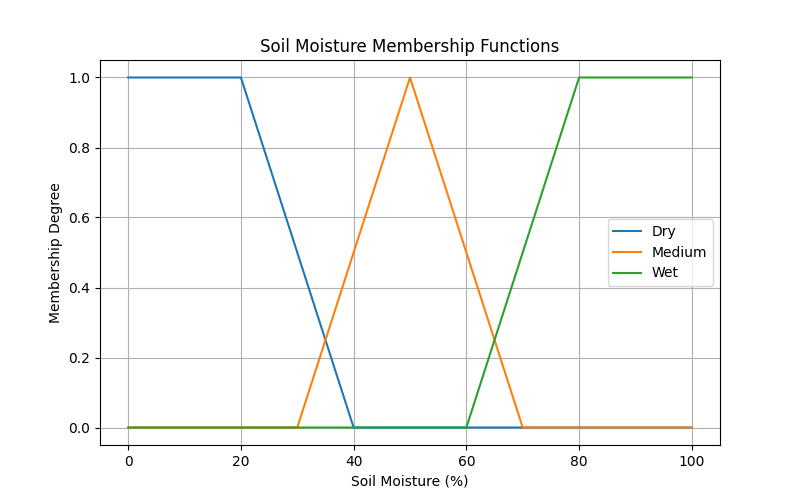
\includegraphics[width=0.8\textwidth]{soil_membership.png}
		\caption{توابع عضویت رطوبت خاک}
		\label{fig:soil_membership}
	\end{figure}
	\begin{figure}[h]
		\centering
		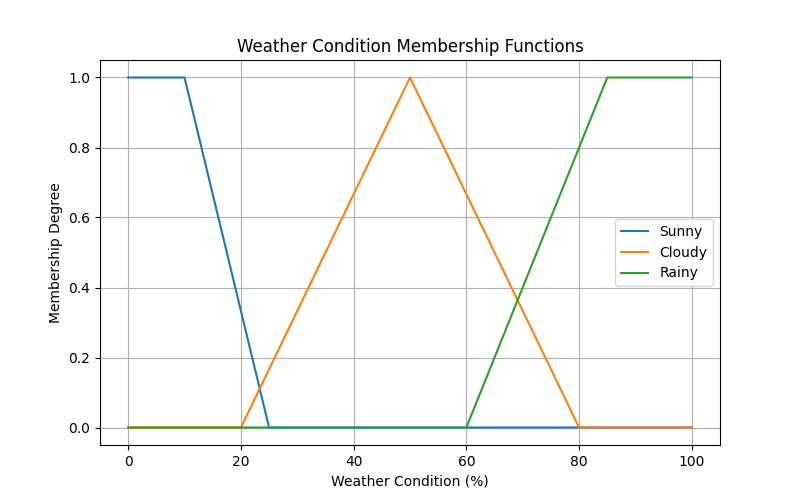
\includegraphics[width=0.8\textwidth]{weather_membership.png}
		\caption{توابع عضویت شرایط جوی}
		\label{fig:weather_membership}
	\end{figure}
	\begin{figure}[h]
		\centering
		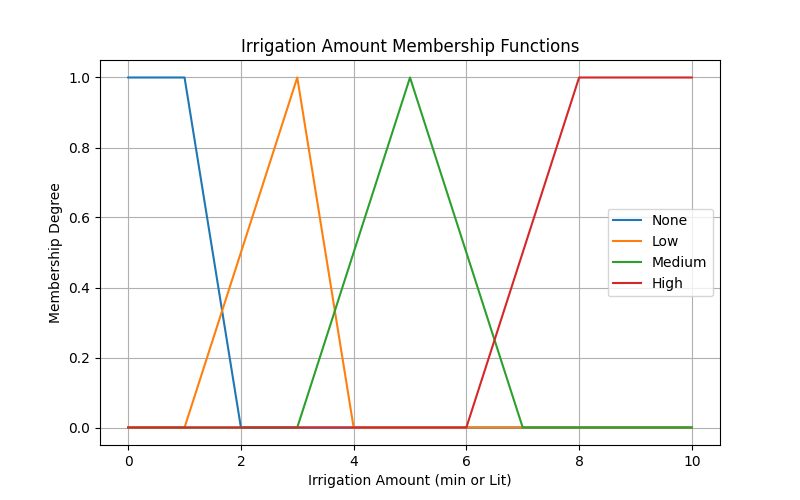
\includegraphics[width=0.8\textwidth]{irrigation_membership.png}
		\caption{توابع عضویت مقدار آبیاری}
		\label{fig:irrigation_membership}
	\end{figure}
	\begin{figure}[h]
		\centering
		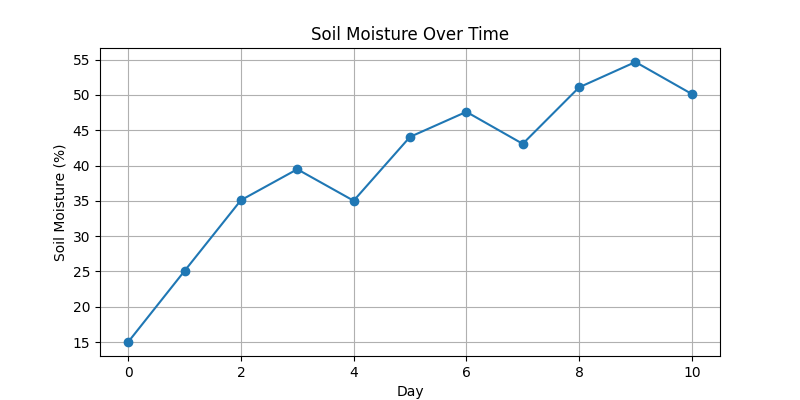
\includegraphics[width=0.8\textwidth]{soil_simulation.png}
		\caption{رطوبت خاک در طول 10 روز شبیه‌سازی}
		\label{fig:soil_simulation}
	\end{figure}
	\begin{figure}[h]
		\centering
		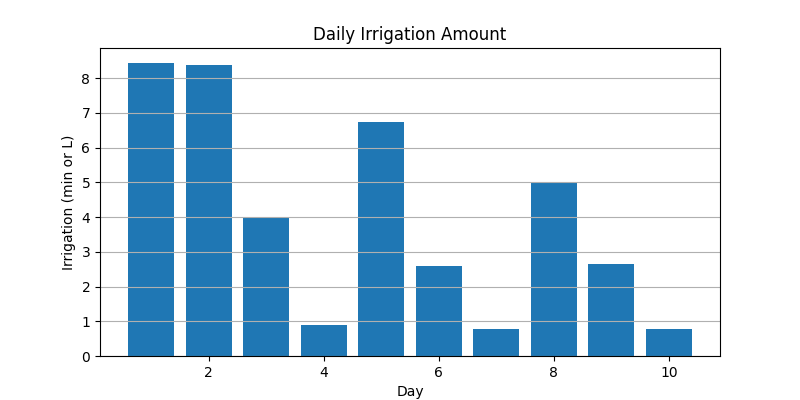
\includegraphics[width=0.8\textwidth]{irrigation_simulation.png}
		\caption{مقدار آبیاری روزانه در شبیه‌سازی}
		\label{fig:irrigation_simulation}
	\end{figure}
	
	

\end{document}